\begin{tikzpicture}[
    node distance = 1cm and 2cm,
    actor/.style={scale=0.5},
    usecase/.style={ellipse, draw, minimum width=4cm, minimum height=0.7cm, align=center, font=\small},
    link/.style={draw, thick}
]

% System Boundary
\draw[thick] (0, 0) rectangle (9, -16);
\node at (4.5, -0.5) {\textbf{Registrar Office Management}};

% Actors
\node (registrar) at (-2, -7.5) {
    \begin{tikzpicture}[scale=0.5]
        \draw[thick] (0,1.2) circle (0.4cm);
        \draw[thick] (0,0.8) -- (0,-0.8);
        \draw[thick] (-0.8,0.4) -- (0.8,0.4);
        \draw[thick] (0,-0.8) -- (-0.5,-1.8);
        \draw[thick] (0,-0.8) -- (0.5,-1.8);
        \node at (0,-2.5) {\small Registrar Office};
    \end{tikzpicture}
};

\node (admin) at (11, -7.5) {
    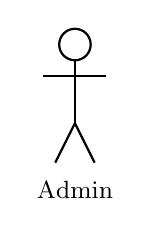
\begin{tikzpicture}[scale=0.5]
        \draw[thick] (0,1.2) circle (0.4cm);
        \draw[thick] (0,0.8) -- (0,-0.8);
        \draw[thick] (-0.8,0.4) -- (0.8,0.4);
        \draw[thick] (0,-0.8) -- (-0.5,-1.8);
        \draw[thick] (0,-0.8) -- (0.5,-1.8);
        \node at (0,-2.5) {\small Admin};
    \end{tikzpicture}
};

% Use Cases
\node[usecase] (uc1) at (4.5, -1.5) {Search Applicant};
\node[usecase] (uc2) at (4.5, -2.5) {Show Applicant Profile};
\node[usecase] (uc3) at (4.5, -3.5) {Receive Documents};
\node[usecase] (uc4) at (4.5, -4.5) {Admit Applicant};
\node[usecase] (uc5) at (4.5, -5.5) {View All Applicants};
\node[usecase] (uc6) at (4.5, -6.5) {View Waited Applicants};
\node[usecase] (uc7) at (4.5, -7.5) {View Admitted Applicants};
\node[usecase] (uc8) at (4.5, -8.5) {Export Applicant List};
\node[usecase] (uc9) at (4.5, -9.5) {Update Applicant Info};
\node[usecase] (uc10) at (4.5, -10.5) {View Pending Documents};
\node[usecase] (uc11) at (4.5, -11.5) {Receive Pending Documents};
\node[usecase] (uc12) at (4.5, -12.5) {Seat Status};
\node[usecase] (uc13) at (4.5, -13.5) {Export Lists};
\node[usecase] (uc14) at (4.5, -14.5) {Create New Record};

% Connections
\foreach \i in {uc1,uc2,uc3,uc4,uc5,uc6,uc7,uc8,uc10,uc11,uc12,uc13}
    \draw[link] (registrar) -- (\i.west);

\draw[link] (admin) -- (uc9.east);
\draw[link] (admin) -- (uc4.east);
\draw[link] (admin) -- (uc14.east);

\end{tikzpicture}